\chapter{Plug-and-Play Priors and Regularisation by Denoising}
\label{ch:pnp}

In Chapter \ref{ch:reg}, we established the framework of variational regularisation, where inverse problems are solved by minimising a functional composed of a data-fidelity term and a regularisation term $J(u)$. In Chapter \ref{chap:nn_reg}, we explored how to learn these regularisers $J_\Theta(u)$ using neural networks (e.g., the NETT framework).

This chapter introduces a different paradigm that bridges the gap between classical optimisation and deep learning: \emph{Plug-and-Play (PnP)} methods. Instead of training a network to be a regulariser $J(u)$, we observe that the ``proximal operator'' step in many optimisation algorithms that we introduced in Chapter \ref{ch:unrolling} is mathematically equivalent to a denoising problem. This allows us to ``plug in'' off-the-shelf image denoisers (such as BM3D or deep neural networks) directly into iterative algorithms, effectively using the denoiser as an implicit prior.

We will explore the PnP framework, its extension to \emph{Regularisation by Denoising (RED)}, and the theoretical challenges regarding the existence of the underlying objective function. Finally, we will connect these methods to modern generative models via \emph{Tweedie's formula} and score matching.

\section{From Proximal Splitting to Plug-and-Play}
\label{sec:pnp_basics}

To understand PnP, we must first revisit the splitting algorithms introduced in Chapter \ref{ch:unrolling}, specifically those designed to solve the standard variational problem \eqref{eq:var_reg}, i.e.
\begin{align}
    u^* \in \argmin_{u} \left\{ F(Ku, f^\delta) + \alpha J(u) \right\} \, .
    \label{eq:pnp_variational}
\end{align}
When $J(u)$ is non-smooth (e.g., Total Variation), we often rely on variable splitting techniques as we have seen in Chapter \ref{ch:unrolling}, where we utilised ADMM and PDHG as primary splitting methods. One splitting method that we haven't discussed is the so-called half-quadratic splitting that we introduce in the next section.

\subsection{Half-Quadratic Splitting (HQS)}
One of the simplest splitting methods is Half-Quadratic Splitting (HQS). We introduce an auxiliary variable $v$ and constrain it to be close to $u$. The problem \eqref{eq:pnp_variational} is reformulated as
\begin{align}
    \min_{u, v} \left\{ F(Ku, f^\delta) + \alpha J(v) + \frac{\mu}{2} \|u - v\|_2^2 \right\} \, ,\label{eq:hqs1}
\end{align}
where $\mu > 0$ is a penalty parameter. As $\mu \to \infty$, the solution converges to that of the original problem. We note the similarities to the ADMM Algorithm \ref{alg:admm}, where now instead of enforcing the constraint $u = v$, we `only' penalise it. Similar to ADMM, we solve \eqref{eq:hqs1} via alternating minimisation, i.e.,
\begin{subequations}
\begin{align}
    u_{k+1} &= \argmin_{u} \left\{ F(Ku, f^\delta) + \frac{\mu}{2} \|u - v_k\|_2^2 \right\} \, , \label{eq:hqs_inversion} \\
    v_{k+1} &= \argmin_{v} \left\{ \frac{\mu}{2} \|u_{k+1} - v\|_2^2 + \alpha J(v) \right\} \, . \label{eq:hqs_denoising}
\end{align}\label{eq:hqs2}%
\end{subequations}
We see that we decouple \eqref{eq:hqs2} into two sub-problems, where one involves the data term and the forward model, but the other one only involves a proximal step: 
\begin{itemize}
    \item \textbf{Step \eqref{eq:hqs_inversion} (Inversion Step):} This is a quadratic problem involving the forward operator $K$. For Gau\ss ian noise (where we have the quadratic data fidelity $F(Ku, f^\delta) = \frac{1}{2}\|Ku - f^\delta\|_2^2$), this step amounts to solving a linear system of equations:
    \[ u_{k+1} = (K^*K + \mu I)^{-1} (K^*f^\delta + \mu v_k) \, . \]
    \item \textbf{Step \eqref{eq:hqs_denoising} (Proximal Step):} By dividing the objective by $\mu$, we recognise this as the definition of the proximal operator for the function $\frac{\alpha}{\mu} J$:
    \[ v_{k+1} = \operatorname{prox}_{\frac{\alpha}{\mu} J} (u_{k+1}) = \argmin_{v} \left\{ \frac{1}{2} \|v - u_{k+1}\|_2^2 + \frac{\alpha}{\mu} J(v) \right\} \, . \]
\end{itemize}
The key benefit of HQS is that we have decoupled the possible non-linearity of the regularisation function(al) $J$ from the forward operator $K$, and reduced the original problem \eqref{eq:hqs1} to a sequence of linear systems solutions and proximal steps. We know that proximal maps as defined in Definition \ref{def:prox_operator}, are solving variational regularisation problems \eqref{eq:var_reg} for the case where the data fidelity term is a quadratic (implying Gau\ss ian noise), and where $K$ is set to be the identity. Hence, in practice, solving \eqref{eq:hqs_denoising} is what we refer to as a \emph{denoising problem}.

\subsection{The Plug-and-Play Heuristic}
The key insight of \cite{venkatakrishnan2013plug} is that the proximal step \eqref{eq:hqs_denoising} is structurally identical to a Gau\ss ian denoising problem. It asks for a vector $v$ that is close to the noisy input $u_{k+1}$ (in the $\ell^2$ sense) but regularised by $J(v)$.

If we interpret $J(v)$ as a negative log-prior ($J(v) = -\log p(v)$), then \eqref{eq:hqs_denoising} is the Maximum A-Posteriori (MAP) estimate of $v$ given the observation $u_{k+1}$ with noise variance $\sigma^2 = \alpha/\mu$.

The PnP strategy now is simple: instead of mathematically deriving the proximal operator for a specific $J$, we replace the proximal operator with a general, state-of-the-art denoising operator $D_\sigma(\cdot)$ that does not need to be a proximal map, i.e. we replace \eqref{eq:hqs_denoising} with
\begin{align}
    v_{k+1} = D_{\sigma_k}(u_{k+1}) \, .
    \label{eq:pnp_update}
\end{align}
The denoiser $D_\sigma$ is usually chosen to be a classical algorithm like BM3D \cite{dabov2007image} or Non-Local Means \cite{buades2005non}, or a trained Deep Neural Network (e.g., DnCNN \cite{zhang2017beyond}, DRUNet \cite{zhang2021plug}).

\section{PnP Algorithms: HQS and ADMM}
\label{sec:pnp_algos}

We can apply this heuristic to any of the various splitting algorithms introduced in Chapter \ref{ch:unrolling} and beyond. Here we detail two of the most common variants.

\subsection{PnP-HQS}
Half-Quadratic Splitting is often chosen for PnP in combination with deep learning-based denoisers because of its simplicity. If we replace \eqref{eq:hqs_denoising} with \eqref{eq:pnp_update} and assume $F(Ku, f^\delta) = \frac12 \| Ku - f^\delta \|^2$, we obtain our first PnP algorithm, outlined in Algorithm \ref{alg:pnphqs}.

\begin{algorithm}
\caption{Plug-and-Play HQS}
\begin{algorithmic}[1]
\State \textbf{Input:} Data $f^\delta$, Forward Operator $K$, Denoiser $D_\sigma$, Parameters $\mu, \alpha$
\State \textbf{Initialise:} $v_0 = f^\delta$, $u_0 = K^\ast f^\delta$
\For{$k = 1, \dots, N$}
    \State
    \State \textbf{1. Inversion:}
    \State $u_{k+1} = \argmin_u \frac{1}{2}\|Ku - f^\delta\|_2^2 + \frac{\mu}{2}\|u - v_k\|_2^2$
    \State
    \State \textbf{2. Denoising:}
    \State $\sigma = \sqrt{\alpha / \mu}$
    \State $v_{k+1} = D_{\sigma}(u_{k+1})$
    \State
\EndFor
\State \textbf{Return:} $u_{N}$
\end{algorithmic}\label{alg:pnphqs}
\end{algorithm}

\subsection{PnP-ADMM}
The Alternating Direction Method of Multipliers (ADMM) as introduced in Algorithm \ref{alg:admm} provides stronger convergence guarantees for convex problems and handles constraints properly and avoids the common pitfalls of penalty methods, such that in practice one has to increase the penalty parameter $\mu$ in order to enforce the constraint $u = v$. For \eqref{eq:pnp_variational} with $F(Ku, f^\delta) = \frac12 \| Ku - f^\delta \|^2$, the corresponding augmented Lagrangian reads
\begin{align*}
    \mathcal{L}_\mu(u, v; w) = \frac12 \| Ku - f^\delta \|^2 + \alpha J(v) + \mu \langle w, u - v \rangle + \frac{\mu}{2} \| u - v \|^2 \, ,
\end{align*}
where we have substituted the original Lagrange multiplier directly with $\mu^{-1} w$. Then the ADMM updates are
\begin{align*}
    u_{k+1} &= (K^*K + \mu I)^{-1} (K^*f^\delta + \mu (v_k -  w_k)) \, , \\
    v_{k+1} &= \operatorname{prox}_{\frac{\alpha}{\mu} J}(u_{k + 1} + w_k) \, , \\
    w_{k+1} &= w_k + (u_{k+1} - v_{k+1}) \, .
\end{align*}
Now, in analogy to the HQS example, for PnP we replace the proximal map that acts as a denoiser with a more general denoiser $D_\sigma$, to obtain the PnP-ADMM algorithm presented in Algorithm \ref{alg:pnpadmm}.
\begin{algorithm}
\caption{Plug-and-Play ADMM}
\begin{algorithmic}[1]
\State \textbf{Input:} Data $f^\delta$, Forward Operator $K$, Denoiser $D_\sigma$, Parameters $\mu, \alpha$
\State \textbf{Initialise:} $u_0 = K^\ast f^\delta$, $v_0 = f^\delta$, $w_0 = 0$
\For{$k = 1, \dots, N$}
    \State
    \State \textbf{1. Inversion:}
    \State $u_{k+1} = (K^*K + \mu I)^{-1} (K^*f^\delta + \mu(v_k - w_k))$
    \State
    \State \textbf{2. Denoising:}
    \State $\sigma = \sqrt{\alpha / \mu}$
    \State $v_{k+1} = D_{\sigma}(u_{k+1} + w_k)$
    \State
    \State \textbf{3. Dual Update:}
    \State $w_{k+1} = w_k + (u_{k+1} - v_{k+1})$
    \State
\EndFor
\State \textbf{Return:} $u_{N}$
\end{algorithmic}\label{alg:pnpadmm}
\end{algorithm}
Here, the denoiser removes the noise (and the artifacts) from the sum of the primal and the dual variable.

\subsection{Practical Parameter Tuning}
A crucial aspect of PnP is the relationship between the regularisation parameter $\alpha$ and the internal noise level of the denoiser $\sigma$. In theory, for the MAP interpretation to hold, we require $\sigma = \sqrt{\alpha/\mu}$. However, in practice, when using deep denoisers (like DRUNet), it is often beneficial to \textbf{decrease $\sigma$} over iterations. Starting with a large $\sigma$ removes heavy artifacts, while a small $\sigma$ in later iterations refines fine details \cite{zhang2021plug}.

\subsection{Iterative Regularisation and PnP Bregman Iterations}
\label{sec:pnp_bregman}

In the previous section, we noted that in standard PnP methods, decreasing the noise level $\sigma$ over iterations is often necessary. This heuristic acts as a continuation method: a large initial $\sigma$ smooths out noise and poor initialisations, while a shrinking $\sigma$ allows the data fidelity term to gradually restore fine textures and contrast that the denoiser initially washed away. 

However, a more mathematically principled alternative exists to restore these details without artificially decaying $\sigma$. Instead of solving the unconstrained variational problem \eqref{eq:pnp_variational}, we can target the strictly constrained formulation
\begin{align}
    \min_{u, v} J(v) \quad \text{subject to} \quad Ku = f^\delta \quad \text{and} \quad u = v \, .
    \label{eq:pnp_constrained}
\end{align}
By applying the method of multipliers to this constrained problem, we introduce two distinct scaled dual variables: the multiplier $w_1$ to enforce data consistency and $w_2$ to enforce the variable splitting. The corresponding Augmented Lagrangian reads
\begin{align}
    \mathcal{L}_\mu(u, v; w_1, w_2) = J(v) &+ \frac{\mu}{2} \| Ku - f^\delta + w_1 \|_2^2 + \frac{\mu}{2} \| u - v + w_2 \|_2^2 \, .
    \label{eq:constrained_lagrangian}
\end{align}
Applying the alternating minimisation steps of ADMM to \eqref{eq:constrained_lagrangian} yields a powerful variant of PnP, which we outline in Algorithm \ref{alg:pnp_constrained_admm}. Taking the gradient of $\mathcal{L}_\mu$ with respect to $u$ and setting it to zero results in the inversion step
\begin{align}
    u_{k+1} = (K^*K + I)^{-1} \left( K^*(f^\delta - w_{1,k}) + (v_k - w_{2,k}) \right) \, .
    \label{eq:pnp_bregman_inversion}
\end{align}
The $v$-update isolates the prior $J$ into a proximal operator, exactly as in standard PnP-ADMM, which we substitute with our off-the-shelf denoiser $D_\sigma$, i.e.,
\begin{align}
    v_{k+1} = D_\sigma(u_{k+1} + w_{2,k}) \, .
    \label{eq:pnp_bregman_denoising}
\end{align}

\begin{algorithm}
\caption{Plug-and-Play Constrained ADMM (PnP-Bregman)}
\begin{algorithmic}[1]
\State \textbf{Input:} Data $f^\delta$, Forward Operator $K$, Denoiser $D_\sigma$, Parameter $\mu$, Tolerance $\tau$
\State \textbf{Initialise:} $u_0 = K^\ast f^\delta$, $v_0 = f^\delta$, $w_1 = 0$, $w_2 = 0$
\For{$k = 1, \dots, N$}
    \State
    \State \textbf{1. Inversion (with Bregman correction):}
    \State $u_{k+1} = (K^*K + I)^{-1} \big( K^*(f^\delta - w_{1,k}) + (v_k - w_{2,k}) \big)$
    \State
    \State \textbf{2. Denoising:}
    \State $v_{k+1} = D_{\sigma}(u_{k+1} + w_{2,k})$
    \State
    \State \textbf{3. Dual Updates:}
    \State $w_{1, k+1} = w_{1, k} + (K u_{k+1} - f^\delta)$
    \State $w_{2, k+1} = w_{2, k} + (u_{k+1} - v_{k+1})$
    \State
    \State \textbf{4. Early Stopping Check:}
    \If{$\|Ku_{k+1} - f^\delta\|_2^2 \le \tau \sigma_{\text{noise}}^2$}
        \State \textbf{break}
    \EndIf
\EndFor
\State \textbf{Return:} $u_{k+1}$
\end{algorithmic}\label{alg:pnp_constrained_admm}
\end{algorithm}

The critical difference in this constrained formulation lies in the dual variable $w_1$. In standard PnP-ADMM, the data fidelity target is fixed at $f^\delta$. Here, $w_1$ acts as a \emph{Bregman iteration} component, continuously integrating the data residual $(Ku - f^\delta)$. This systematically re-injects lost contrast and high-frequency details back into the inversion step \eqref{eq:pnp_bregman_inversion} to strictly enforce the forward model. 

Because the algorithm dynamically compensates for over-smoothing via $w_1$, one can typically operate the denoiser at a \textbf{fixed} noise level $\sigma$, significantly simplifying hyperparameter tuning. Furthermore, because this algorithm seems to force $Ku \to f^\delta$ as $k \to \infty$, it represents an \emph{iterative regularisation} method. If run to infinity on noisy data, it will eventually fit the noise.  Therefore, early stopping is strictly required; in practice, we halt the iteration using Morozov's discrepancy principle \cite{morozov1966solution} as soon as the residual drops below the known noise level $\| f - f^\delta \|$.

\section{Theoretical Guarantees and Convergence of PnP}
\label{sec:pnp_convergence}

While the empirical success of Plug-and-Play methods is undeniable, establishing rigorous mathematical guarantees for their convergence remains a highly active area of research. In classical splitting methods (like standard ADMM or HQS), convergence proofs rely heavily on the assumption that the regularisation term $J$ is a proper, closed, and convex function. 

In such classical proofs, the proximal operator step involves finding the resolvent of a monotone operator (specifically, the subdifferential $\partial J$). This monotonicity guarantees that the dual and primal updates form a non-expansive sequence, allowing one to construct a Lyapunov sequence that monotonously decreases, proving that the algorithm targets a saddle point of the Augmented Lagrangian.

However, when we replace the proximal step with an off-the-shelf denoiser $D_\sigma(\cdot)$, we fundamentally break this assumption. Most state-of-the-art denoisers do not correspond to the proximal operator of any underlying regularisation functional $J$. Consequently, the sequence of iterations is no longer guaranteed to minimise a global objective function. To recover convergence guarantees, the literature generally splits into two distinct paradigms: the \emph{Optimisation Perspective} and the \emph{Fixed-Point Perspective}.

\subsection{The Optimisation Perspective: Enforcing Proximal Behaviour}
To preserve the classical convergence proofs, one must ensure that the chosen denoiser $D_\sigma$ mathematically behaves like a proximal operator. By Moreau's Theorem, a function $D_\sigma: \mathbb{R}^n \to \mathbb{R}^n$ is the proximal operator of some closed, proper, convex function $J$ if and only if it satisfies two conditions:
\begin{enumerate}
    \item \textbf{Non-expansiveness:} $D_\sigma$ must be Lipschitz continuous with a Lipschitz constant $L \le 1$.
    \item \textbf{Symmetric Jacobian:} The Jacobian matrix $\nabla D_\sigma(x)$ must be symmetric for all $x$. 
\end{enumerate}

The symmetry of the Jacobian is equivalent to stating that $D_\sigma$ forms a conservative vector field, meaning it is the gradient of some scalar potential function. As highlighted in recent literature (cf. \cite{reehorst2018regularization}), standard denoisers such as BM3D, Non-Local Means, and typical convolutional neural networks (CNNs) exhibit highly non-symmetric Jacobians. Therefore, they cannot be interpreted as minimising a regularised objective. 

To resolve this, recent works have proposed designing specific neural network architectures that structurally guarantee a symmetric Jacobian and bounded Lipschitz constants. If such a tailored denoiser is used, PnP-ADMM and PnP-HQS mathematically reduce to standard splitting methods, and classical convergence to a global objective minimum is guaranteed.

\subsection{The Fixed-Point Perspective: Convergence of PnP-HQS}
If we abandon the requirement that an underlying objective function $J$ exists, we can no longer frame PnP as an optimisation algorithm. Instead, we must analyse it as a sequence of operator compositions and rely on fixed-point theory. Here, the goal is not to find a minimum, but rather a \emph{fixed point} $v^* = T(v^*)$ representing a state of ``consensus equilibrium'' between the data fidelity and the denoiser.

This approach is particularly elegant for PnP-HQS. Let us define the data fidelity functional as $G(u) = F(Ku, f^\delta)$. The inversion step \eqref{eq:hqs_inversion} of PnP-HQS is exactly the proximal operator of $G$ scaled by $1/\mu$, i.e.,
\begin{align}
    u_{k+1} &= \operatorname{prox}_{G/\mu}(v_k) \, . \label{eq:hqs_prox_G}
\end{align}
Substituting this into the denoising step \eqref{eq:pnp_update}, the entire PnP-HQS algorithm can be written as a single, explicit operator iteration $v_{k+1} = T(v_k)$, where
\begin{align}
    T = D_\sigma \circ \operatorname{prox}_{G/\mu} \, .
    \label{eq:pnp_hqs_operator}
\end{align}

To guarantee that the sequence $\{v_k\}$ converges to a fixed point, we rely on the Lipschitz properties of the composed operator $T$. We know from convex analysis that the proximal operator of a closed, convex function $G$ is firmly non-expansive, meaning its Lipschitz constant is $L_{\text{prox}} \le 1$. The convergence of $T$ then depends entirely on the Lipschitz constant of the denoiser, $L_D$:
\begin{itemize}
    \item \textbf{Strict Contraction (Banach Fixed-Point Theorem):} If the denoiser is trained or constrained to be a \emph{strict contraction} ($L_D < 1$), then the composition $T$ is also a strict contraction ($L_T \le L_D L_{\text{prox}} < 1$). By the \href{https://en.wikipedia.org/wiki/Banach_fixed-point_theorem}{Banach Fixed-Point Theorem}, the PnP-HQS iteration $v_{k+1} = T(v_k)$ is guaranteed to converge to a unique fixed point $v^*$ for any initialisation $v_0$.
    \item \textbf{Non-Expansive (Krasnosel'skii-Mann Theorem):} If the denoiser is only non-expansive ($L_D = 1$), the operator $T$ is non-expansive ($L_T = 1$). In this case, standard iterations may oscillate. However, convergence to a fixed point can still be guaranteed by employing the Krasnosel'skii-Mann (KM) theorem, which requires applying an averaging step (or relaxation) to the operator
    \begin{align}
        v_{k+1} = (1 - \rho)v_k + \rho T(v_k) \, , \quad \text{for } \rho \in (0, 1) \, .
    \end{align}
\end{itemize}
By ensuring that deep learning denoisers are 1-Lipschitz (e.g., via spectral normalisation during training), researchers can guarantee the robust convergence of PnP-HQS to a consensus equilibrium, even without an underlying objective function.

\section{Regularisation by Denoising (RED)}
\label{sec:red}

One of the primary criticisms of standard Plug-and-Play (PnP) methods is that by merely replacing a proximal operator with an arbitrary denoiser, we break the link to the original variational objective \eqref{eq:pnp_variational}. Without an explicit regularisation functional $J$, it is difficult to characterise what the algorithm is actually minimising, or to define a concrete energy landscape.

\emph{Regularisation by Denoising (RED)}, introduced by \cite{romano2017little}, attempts to bridge this gap by defining an \emph{explicit} regularisation functional that is constructed directly from the application of the chosen denoiser.

\subsection{The RED Functional}
The core idea of RED is to penalise the correlation between the image and the noise extracted by the denoiser. Let $D(u)$ be an off-the-shelf denoiser. The residual $u - D(u)$ can be interpreted as the noise (or high-frequency artifacts) isolated by the denoiser. RED defines the regularisation functional as
\begin{align}
    \rho(u) = \frac{1}{2} \langle u, u - D(u) \rangle \, .
    \label{eq:red_functional}
\end{align}
The intuition is elegant: if $u$ is a clean image, the denoiser should not alter it significantly, meaning $D(u) \approx u$, and thus $\rho(u) \approx 0$. Conversely, if $u$ is noisy or contains severe artifacts, the inner product between the image and the extracted noise will yield a larger penalty.

\subsection{Deriving the RED Gradient}
To use $\rho(u)$ in a variational framework, we formulate the overall objective function as
\begin{align}
    E(u) = F(Ku, f^\delta) + \alpha \rho(u) \, .
    \label{eq:red_objective}
\end{align}
To minimise this using gradient-based methods, we must compute $\nabla \rho(u)$. Applying the product rule to \eqref{eq:red_functional}, we obtain
\begin{align}
    \nabla \rho(u) &= \frac{1}{2} \nabla_u \left( \langle u, u \rangle - \langle u, D(u) \rangle \right) \nonumber \\
    &= \frac{1}{2} \left( 2u - D(u) - [\nabla D(u)]^\top u \right) \nonumber \\
    &= \frac{1}{2} \left( u - D(u) \right) + \frac{1}{2} \left( u - [\nabla D(u)]^\top u \right) \, ,
    \label{eq:red_gradient_expansion}
\end{align}
where $\nabla D(u)$ is the Jacobian matrix of the denoiser $D$. 

In \cite{romano2017little}, the authors claim that under specific conditions, the gradient simplifies to the denoising residual itself, i.e.,
\begin{align}
    \nabla \rho(u) = u - D(u) \, .
    \label{eq:red_gradient_claim}
\end{align}
Looking at \eqref{eq:red_gradient_expansion}, for \eqref{eq:red_gradient_claim} to hold, we strictly require that $[\nabla D(u)]^\top u = D(u)$. The authors justify this via two strong mathematical assumptions about the denoiser:
\begin{enumerate}
    \item \textbf{Jacobian Symmetry:} The denoiser's Jacobian is symmetric, meaning $[\nabla D(u)]^\top = \nabla D(u)$.
    \item \textbf{Local Homogeneity:} The denoiser is locally homogeneous, satisfying $D(cu) = c D(u)$ for a scalar $c$ close to 1. By \href{https://en.wikipedia.org/wiki/Homogeneous_function#Euler's_theorem}{Euler's homogeneous function theorem}, taking the derivative with respect to $c$ yields the directional derivative condition $\nabla D(u) u = D(u)$.
\end{enumerate}
If both conditions are met, then $[\nabla D(u)]^\top u = \nabla D(u) u = D(u)$, and the second term in \eqref{eq:red_gradient_expansion} matches the first, yielding \eqref{eq:red_gradient_claim}. With this simple gradient, one can deploy standard optimisation schemes (like Gradient Descent or ADMM) to minimise the explicitly defined energy $E(u)$. For example, a simple gradient descent update becomes
\begin{align}
    u_{k+1} = u_k - \tau \left( \nabla F(Ku_k, f^\delta) + \alpha (u_k - D(u_k)) \right) \, .\label{eq:red-gd}
\end{align}
In the following, we want discuss how realistic the assumptions of Jacobian symmetry and local homogeneity for denoiser are in practice.

\section{Theoretical Analysis and The Jacobian Critique}
\label{sec:pnp_critique}

The RED framework presents an attractive narrative: it offers the flexibility of PnP while maintaining the mathematical rigorousness of explicit variational regularisation. However, a detailed analysis by \cite{reehorst2018regularization} revealed a fundamental flaw in the foundational assumptions of RED when applied to practical denoisers.

\subsection{The Vector Field and Symmetry Condition}
For an iterative algorithm updating via $u_{k+1} = u_k - \tau V(u_k)$ to be minimising a scalar objective function $\rho(u)$, the vector field $V(u)$ must be \href{https://en.wikipedia.org/wiki/Conservative_vector_field}{\emph{conservative}}. Mathematically, $V(u)$ must be the exact gradient of some scalar potential. 

A fundamental theorem of vector calculus states that a continuously differentiable vector field $V$ is conservative if and only if its Jacobian matrix is symmetric. In the context of RED, the proposed gradient vector field is $V(u) = u - D(u)$. The Jacobian of this field is
\begin{align*}
    \nabla V(u) = I - \nabla D(u) \, .
\end{align*}
Therefore, for $u - D(u)$ to be the gradient of \emph{any} scalar function, the denoiser's Jacobian $\nabla D(u)$ must be symmetric, i.e.,
\begin{align}
    \frac{\partial [D(u)]_i}{\partial u_j} = \frac{\partial [D(u)]_j}{\partial u_i} \quad \text{for all } i, j \, .
    \label{eq:symmetry_condition}
\end{align}
In the following, we briefly discuss how realistic the assumption \eqref{eq:symmetry_condition} is for general denoisers.

\subsection{Reality Check: Do Denoisers have Symmetric Jacobians?}
The authors in \cite{reehorst2018regularization} conducted rigorous tests to determine if modern, off-the-shelf denoisers exhibit symmetric Jacobians. Their findings were definitive:
\begin{itemize}
    \item \textbf{Classical Denoisers:} Algorithms like Non-Local Means (NLM) and BM3D are highly non-linear and rely on complex, data-dependent block-matching mechanisms. Consequently, their Jacobians are highly asymmetric.
    \item \textbf{Deep Learning Denoisers (CNNs):} Standard feed-forward networks (e.g., DnCNN, UNet) involve interleaved convolutions and non-linear activations (like ReLU). Unless specific architectural constraints are enforced (as discussed previously in Section \ref{sec:pnp_convergence}), neural network Jacobians are entirely non-symmetric.
\end{itemize}
\textbf{The Consequence:} Because $\nabla D(u)$ is not symmetric for practical denoisers, the vector field $u - D(u)$ has a non-zero curl. It is not conservative, and therefore, it is \textbf{not the gradient of $\rho(u)$}, nor is it the gradient of any other scalar functional. The elegant RED objective \eqref{eq:red_objective} is a phantom function; the RED algorithms do not actually minimise it.

\subsection{Consensus Equilibrium}
If standard RED algorithms (and standard PnP methods) are not minimising a cost function, how do we mathematically characterise their stationary points?

Instead of viewing these methods through the lens of optimisation, \cite{reehorst2018regularization} and subsequent works suggest interpreting them through the lens of \textbf{Consensus Equilibrium}. The algorithms are essentially root-finding methods attempting to solve the system of non-linear equations
\begin{align}
    \nabla F(Ku^*, f^\delta) + \alpha (u^* - D(u^*)) = 0 \, .\label{eq:red-fixed-point}
\end{align}
At a stationary point $u^*$, the algorithm achieves an equilibrium between two competing vector fields. The forward model gradient $\nabla F(Ku^*, f^\delta)$ pulls the solution towards data consistency, while the denoising residual $(u^* - D(u^*))$ pulls the solution towards the manifold of natural images as implicitly defined by the denoiser. 

While they do not descend an explicit energy landscape, algorithms that seek this consensus equilibrium remain highly effective and represent the true mathematical nature of unconstrained Plug-and-Play and RED methods.

\subsection{Practical RED Algorithms}
\label{sec:red_algorithms}

While a naive gradient descent approach can be used to seek the consensus equilibrium, \cite{romano2017little} proposed more efficient solvers. The most notable is the \emph{Fixed-Point RED (FP-RED)} algorithm. If we assume a Gau\ss ian noise model where $F(Ku, f^\delta) = \frac{1}{2}\|Ku - f^\delta\|_2^2$, the stationary point condition for RED, \eqref{eq:red-fixed-point}, reads
\begin{align}
    K^*(Ku^* - f^\delta) + \alpha (u^* - D(u^*)) = 0 \, .
\end{align}
By rearranging the terms to isolate one instance of $u^*$ on the left-hand side, we obtain a fixed-point equation
\begin{align}
    (K^*K + \alpha I) u^* = K^* f^\delta + \alpha D(u^*) \, .
\end{align}
This naturally suggests an iterative fixed-point scheme, where we evaluate the denoiser at the current iterate $u_k$ and solve the resulting linear system for the next iterate $u_{k+1}$:
\begin{align}
    u_{k+1} = (K^*K + \alpha I)^{-1} \left( K^* f^\delta + \alpha D(u_k) \right) \, .
    \label{eq:fp_red}
\end{align}

Notice the striking structural similarity between FP-RED \eqref{eq:fp_red} and the inversion step of PnP-HQS \eqref{eq:hqs_inversion}. Both algorithms require solving a Tikhonov-regularised linear system at each step. However, while PnP-HQS applies the denoiser sequentially \emph{after} the inversion step, FP-RED integrates the denoiser's output directly into the source term of the linear inversion. 

The authors of \cite{romano2017little} also introduced an ADMM variant of RED. Similar to PnP, variable splitting is introduced ($u = v$), but instead of replacing a proximal operator, the RED residual $(v - D(v))$ is explicitly evaluated within the $v$-update sub-problem.

\subsection{Convergence of RED as Root-Finding}
\label{sec:red_convergence}

Because we established in Section \ref{sec:pnp_critique} that RED algorithms do not minimise a global objective function, we cannot rely on standard descent lemmas to prove their convergence. We must evaluate FP-RED as a root-finding sequence solving a consensus equilibrium.


Fortunately, the authors in \cite{reehorst2018regularization} demonstrated that even without the symmetric Jacobian assumption, FP-RED can be rigorously proven to converge using monotone operator theory. Let us define the FP-RED update \eqref{eq:fp_red} as an operator $T_{FP}$, i.e.,
\begin{align}
    u_{k+1} = T_{FP}(u_k) \quad \text{where} \quad T_{FP}(u) = (K^*K + \alpha I)^{-1} (K^* f^\delta + \alpha D(u)) \, .
\end{align}
The linear inversion operator $(K^*K + \alpha I)^{-1}$ is firmly non-expansive, acting as a dampening factor. Therefore, the convergence of the entire sequence relies entirely on the Lipschitz continuity of the denoiser $D(u)$:
\begin{itemize}
    \item If the denoiser is a \textbf{strict contraction} (Lipschitz constant $L_D < 1$), then $T_{FP}$ is also a strict contraction. By the Banach Fixed-Point Theorem, FP-RED converges to a unique consensus equilibrium regardless of initialisation.
    \item If the denoiser is \textbf{non-expansive} ($L_D \le 1$), $T_{FP}$ is non-expansive. While standard iterations might theoretically oscillate, applying a slight relaxation (averaging the current step with the previous step) guarantees convergence to a fixed point via the Krasnosel'skii-Mann (KM) theorem.
\end{itemize}
Thus, the theoretical requirement for RED to stably converge is identical to that of PnP-HQS: we must constrain the denoiser to be non-expansive. In deep learning architectures, this is typically achieved using spectral normalisation techniques during training. As long as this Lipschitz constraint is satisfied, RED serves as a robust, mathematically convergent root-finding algorithm.

\section{Probabilistic Perspectives: Generative Priors}
\label{sec:tweedie}

Throughout this chapter, we have viewed Plug-and-Play (PnP) and Regularisation by Denoising (RED) primarily through the lens of optimisation and root-finding. We sought MAP (Maximum A-Posteriori) estimates or consensus equilibria. However, this classical optimisation perspective has a potential limitation: finding the MAP estimate is equivalent to finding the single tallest peak (the mode) of a probability landscape, completely ignoring the volume and shape of the surrounding distribution. In highly ambiguous inverse problems, the mode might be fragile or unrepresentative of the broader set of valid solutions.

If we shift our perspective from finding the \emph{mode} of a distribution to finding the \emph{expected value} or \emph{mean} (the Minimum Mean Squared Error, MMSE), a beautiful mathematical equivalence emerges. The expected value acts as the center of mass, balancing the entire probability landscape. 

Crucially, this shift is not just a theoretical exercise; it is strictly connected to how modern deep learning denoisers are trained. When a neural network denoiser is trained using a Mean Squared Error (MSE) loss function over a massive dataset of clean and noisy image pairs, it is penalised quadratically for its mistakes. To minimise this squared penalty across all possible ambiguous observations, a well-known result in statistical decision theory proves that the network is mathematically forced to output the conditional average of all possible clean images that could have produced the noisy input. 

In other words, an optimal MSE denoiser does not compute a MAP estimate; it naturally computes the posterior mean. Recent developments \cite{milanfar2025denoising, tan2025solving} have leveraged this connection to re-establish a more rigorous and elegant link between off-the-shelf denoisers and Bayesian probability theory.

\subsection{Derivation of Tweedie's Formula}

Before diving into what is known as Tweedie's formula, we must first understand how the prior distribution interacts with our noisy observation. In the Bayesian framework, our knowledge about a clean image $x$ given the noisy observation $y$ is captured by the \emph{posterior distribution}, $p(x | y)$. According to Bayes' theorem, the posterior is calculated as
\begin{align}
    p(x | y) = \frac{p(y | x) p(x)}{p(y)} \, ,
    \label{eq:bayes}
\end{align}
where we identify three critical components:
\begin{itemize}
    \item $p(y | x)$ is the \textbf{likelihood}: It models the measurement process and the noise (e.g., the probability of observing $y$ if the true image was exactly $x$).
    \item $p(x)$ is the \textbf{prior}: It encapsulates our belief about the signal before any measurement is taken. For natural images, this dictates how realistic or natural an image $x$ is.
    \item $p(y) = \int p(y | x) p(x) \, dx$ is the \textbf{marginal likelihood} (or evidence), which acts as a normalisation constant.
\end{itemize}

If our goal is to find the Minimum Mean Squared Error (MMSE) estimator, we must compute the expected value (mean) of this posterior distribution, i.e.,
\begin{align*}
    D_\sigma^*(y) = \mathbb{E}[x | y] = \int x \, p(x | y) \, dx = \int x \frac{p(y | x) p(x)}{p(y)} \, dx \, .
\end{align*}
Here lies the fundamental challenge of Bayesian image restoration: the true prior distribution $p(x)$ for natural images is an unimaginably complex, high-dimensional manifold. Because we cannot write down a simple mathematical formula for $p(x)$, analytically solving this integral is strictly impossible.

However, a profound result from statistics known as \textbf{Tweedie's Formula} proves that we can completely bypass the need to know $p(x)$. Assume the signal is corrupted by additive white Gau\ss ian noise $n \sim \mathcal{N}(0, \sigma^2 I)$, so the likelihood is purely Gau\ss ian, i.e.,
\begin{align*}
    p(y | x) = \frac{1}{(2\pi\sigma^2)^{N/2}} \exp\left( - \frac{\|y - x\|_2^2}{2\sigma^2} \right) \, .
\end{align*}
Taking the gradient of the likelihood with respect to the observation $y$ yields
\begin{align}
    \nabla_y p(y | x) = -\frac{y - x}{\sigma^2} p(y | x) \, .
    \label{eq:tweedie_likelihood_grad}
\end{align}
Now, we consider the marginal distribution of the noisy data, $p_\sigma(y)$, obtained by marginalising out $x$:
\begin{align}
    p_\sigma(y) = \int p(y | x) p(x) \, dx \, .\label{eq:marginalised_noisy_data_distribution}
\end{align}
Let us take the gradient of \eqref{eq:marginalised_noisy_data_distribution} with respect to $y$. We can move the gradient inside the integral due to linearity and substitute \eqref{eq:tweedie_likelihood_grad} to obtain
\begin{align}
    \nabla_y p_\sigma(y) &= \int \nabla_y p(y | x) p(x) \, dx \nonumber \\
    &= \int \left( -\frac{y - x}{\sigma^2} \right) p(y | x) p(x) \, dx \, .
\end{align}
Using Bayes' rule, we know that $p(y | x) p(x) = p(x | y) p_\sigma(y)$. Substituting this into the integral yields
\begin{align}
    \nabla_y p_\sigma(y) &= -\frac{1}{\sigma^2} \int (y - x) p(x | y) p_\sigma(y) \, dx \nonumber \\
    &= -\frac{p_\sigma(y)}{\sigma^2} \left( y \int p(x | y) \, dx - \int x \, p(x | y) \, dx \right) \, .
\end{align}
Since $\int p(x | y) \, dx = 1$ (it is a probability distribution) and the second integral being exactly the posterior mean $\mathbb{E}[x | y]$, we obtain
\begin{align}
    \nabla_y p_\sigma(y) = -\frac{p_\sigma(y)}{\sigma^2} \Big( y - \mathbb{E}[x | y] \Big) \, .
\end{align}
Dividing both sides by $p_\sigma(y)$ and recognising that $\frac{\nabla p}{p} = \nabla \log p$, we arrive at \textbf{Tweedie's Formula}
\begin{align}
    \mathbb{E}[x | y] = y + \sigma^2 \nabla_y \log p_\sigma(y) \, .
    \label{eq:tweedie}
\end{align}
It states that the optimal MMSE denoiser $D_\sigma^*(y) = \mathbb{E}[x | y]$ depends only on the gradient of the log-marginal distribution of the \emph{noisy} data.

\subsection{Resolving the RED Mystery: Score-Matching by Denoising} 
Rearranging \eqref{eq:tweedie}, we can express the \textbf{score function} (the vector field pointing towards higher probability density) directly in terms of the denoiser's residual:
\begin{align}
    \nabla_y \log p_\sigma(y) = \frac{D_\sigma^*(y) - y}{\sigma^2} \, .
    \label{eq:score_denoiser}
\end{align}
This insight completely resolves the theoretical crisis of RED discussed in Section \ref{sec:pnp_critique}. Recall that RED attempted to define a regularisation gradient $\nabla \rho(u) = u - D(u)$. We proved this was not a valid gradient of any explicit functional unless the corresponding Jacobian was symmetric and we made strong assumptions on local homogeneity.

However, the authors of \cite{reehorst2018regularization} pointed out that by applying Tweedie's formula, the RED gradient is actually proportional to the negative score of the data distribution:
\begin{align*}
    u - D(u) = -\sigma^2 \nabla_u \log p_\sigma(u) \, .
\end{align*}
Therefore, RED and PnP are not minimising an arbitrary mathematical energy $\rho(u)$; instead, \textbf{they are performing gradient ascent on the log-probability of the data}. The residual $u - D(u)$ is systematically pushing the iterates towards the high-density regions of the prior distribution. Th authors of \cite{reehorst2018regularization} named this paradigm \emph{Score-Matching by Denoising (SMD)}.

\subsection{From PnP to Diffusion Models: Langevin Dynamics}

Once we understand that a trained neural network denoiser $D_\sigma(u)$ is fundamentally an estimator of the score $\nabla \log p_\sigma(u)$, new mathematical connections and insights can be unlocked. 

Up to this point in the chapter, our iterative algorithms (like PnP and RED) have been completely deterministic. Given a starting image and a noisy observation $f^\delta$, the algorithm climbs the probability landscape until it reaches a single peak (the MAP estimate) or a single point of consensus. 

However, in many inverse problems, the observation $f^\delta$ is highly ambiguous. For instance, if an image is heavily blurred or has missing pixels, there might be dozens of perfectly valid, sharp images that match the observation. Instead of merely finding a single best guess, what if we want to explore all possible solutions? To do this, we need to \emph{sample} from the posterior distribution $p(u | f^\delta)$. 

This is achieved using \textbf{Langevin Dynamics}. Originally developed in physics to model the movement of particles (like pollen) suspended in a fluid, Langevin dynamics describes a system driven by two competing forces: a deterministic pull towards a lower energy state, and a random jostling from thermal noise.

\begin{figure}[htbp]
    \centering
    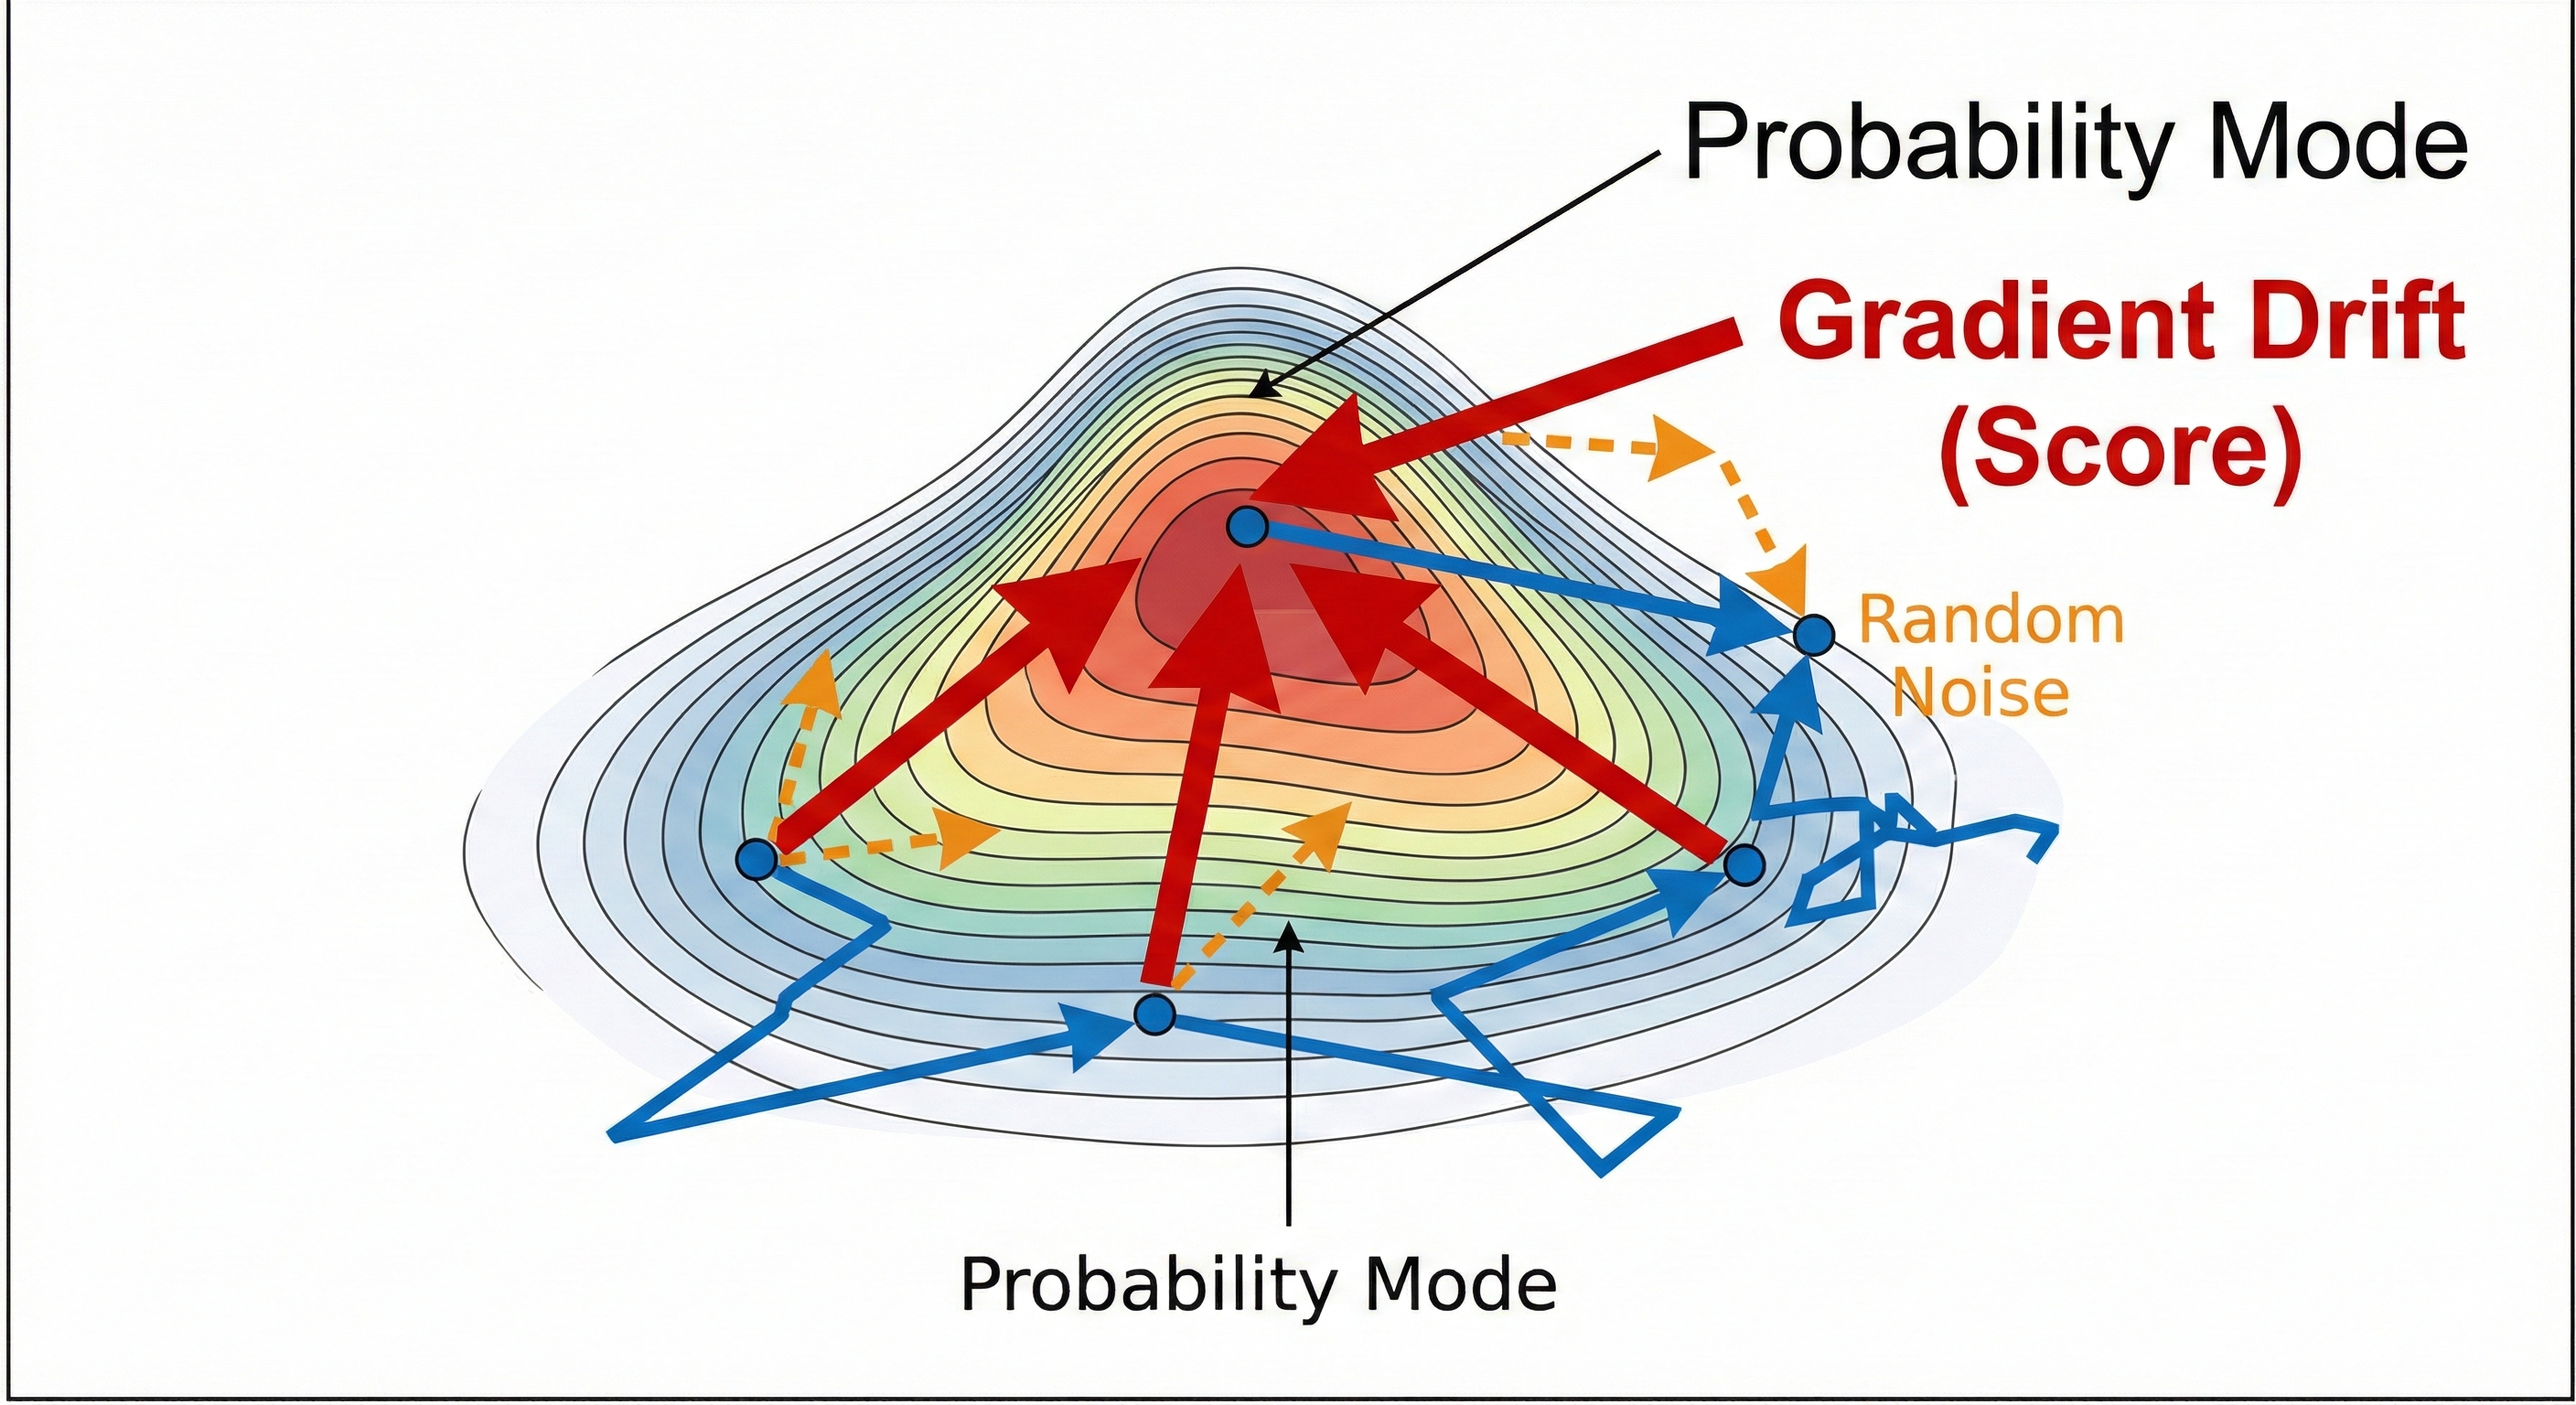
\includegraphics[width=0.9\textwidth]{../Common_Images/pnp/langevin-gradient-drift.png}
    \caption{Illustration of Langevin dynamics: gradient drift pulls the particle toward a high-probability mode while stochastic noise scatters the trajectory. Image generated with Nano Banana Pro.}
    \label{fig:langevin_gradient_drift}
\end{figure}

In the context of probability, we can simulate this physical process to explore our probability distribution. The Langevin dynamics update rule reads
\begin{align}
    u_{k+1} = u_k + \frac{\tau}{2} \nabla_u \log p(u_k | f^\delta) + \sqrt{\tau} z_k \, , \quad \text{where } z_k \sim \mathcal{N}(0, I) \, .
    \label{eq:langevin_base}
\end{align}
Let us break this formula down into its individual parts:
\begin{enumerate}
    \item $u_k$: Our current image guess.
    \item $\frac{\tau}{2} \nabla_u \log p(u_k | f^\delta)$: The \textbf{Gradient Drift}. This is a standard gradient ascent step with step size $\tau/2$. The score $\nabla \log p$ acts as a compass, pointing the image uphill towards higher probability. If we only used this term, we would just climb straight to the single peak.
    \item $\sqrt{\tau} z_k$: The \textbf{Random Noise Injection}. At every step, we add a small amount of random Gau\ss ian noise $z_k$. This noise actively kicks the image off the direct path.
\end{enumerate}
Why add noise? By constantly jostling the image, we prevent it from getting stuck at the exact top of the probability peak. Instead, the image wanders around the high-probability region. By saving the image at different steps, we generate a diversity of valid solutions.

To apply \eqref{eq:langevin_base} to our inverse problem, we need the score of the posterior, $\nabla_u \log p(u | f^\delta)$. We can find this using Bayes' rule (Equation \ref{eq:bayes}), i.e.,
\begin{align*}
    p(u | f^\delta) = \frac{p(f^\delta | u) p(u)}{p(f^\delta)} \, .
\end{align*}
Taking the natural logarithm of both sides turns the multiplication and division into simple addition and subtraction:
\begin{align*}
    \log p(u | f^\delta) = \log p(f^\delta | u) + \log p(u) - \log p(f^\delta) \, .
\end{align*}
Now, we take the gradient with respect to the image $u$. Because the marginal likelihood $p(f^\delta)$ does not depend on the specific image $u$, its gradient is zero and it completely vanishes! This leaves us with
\begin{align}
    \nabla_u \log p(u | f^\delta) = \nabla_u \log p(f^\delta | u) + \nabla_u \log p(u) \, .
    \label{eq:posterior_score_split}
\end{align}
This equation is beautifully intuitive. The direction of highest posterior probability is simply the sum of two separate "compasses":
\begin{enumerate}
    \item $\nabla_u \log p(f^\delta | u)$: The \emph{likelihood score}. This pushes the image to match the physical measurements. If our data fidelity assumes Gau\ss ian noise, this is exactly the negative gradient of our data term, i.e., $-\nabla_u F(Ku, f^\delta)$.
    \item $\nabla_u \log p(u)$: The \emph{prior score}. This pushes the image to look like a natural image. By Tweedie's Formula (Equation \ref{eq:score_denoiser}), we know this is equal to $\frac{1}{\sigma^2}(D_\sigma(u) - u)$.
\end{enumerate}
Substituting these two components back into our Langevin dynamics formula \eqref{eq:langevin_base}, the final sampling update becomes
\begin{align}
    u_{k+1} = u_k - \frac{\tau}{2} \nabla_u F(Ku_k, f^\delta) + \frac{\tau}{2\sigma^2} \Big( D_\sigma(u_k) - u_k \Big) + \sqrt{\tau} z_k \, .
    \label{eq:langevin_pnp}
\end{align}
Note that if we remove the random noise $\sqrt{\tau} z_k$, Equation \eqref{eq:langevin_pnp} is mathematically identical to the gradient descent update for RED \eqref{eq:marginalised_noisy_data_distribution}, and therefore highly related to PnP.

\begin{figure}[htbp]
    \centering
    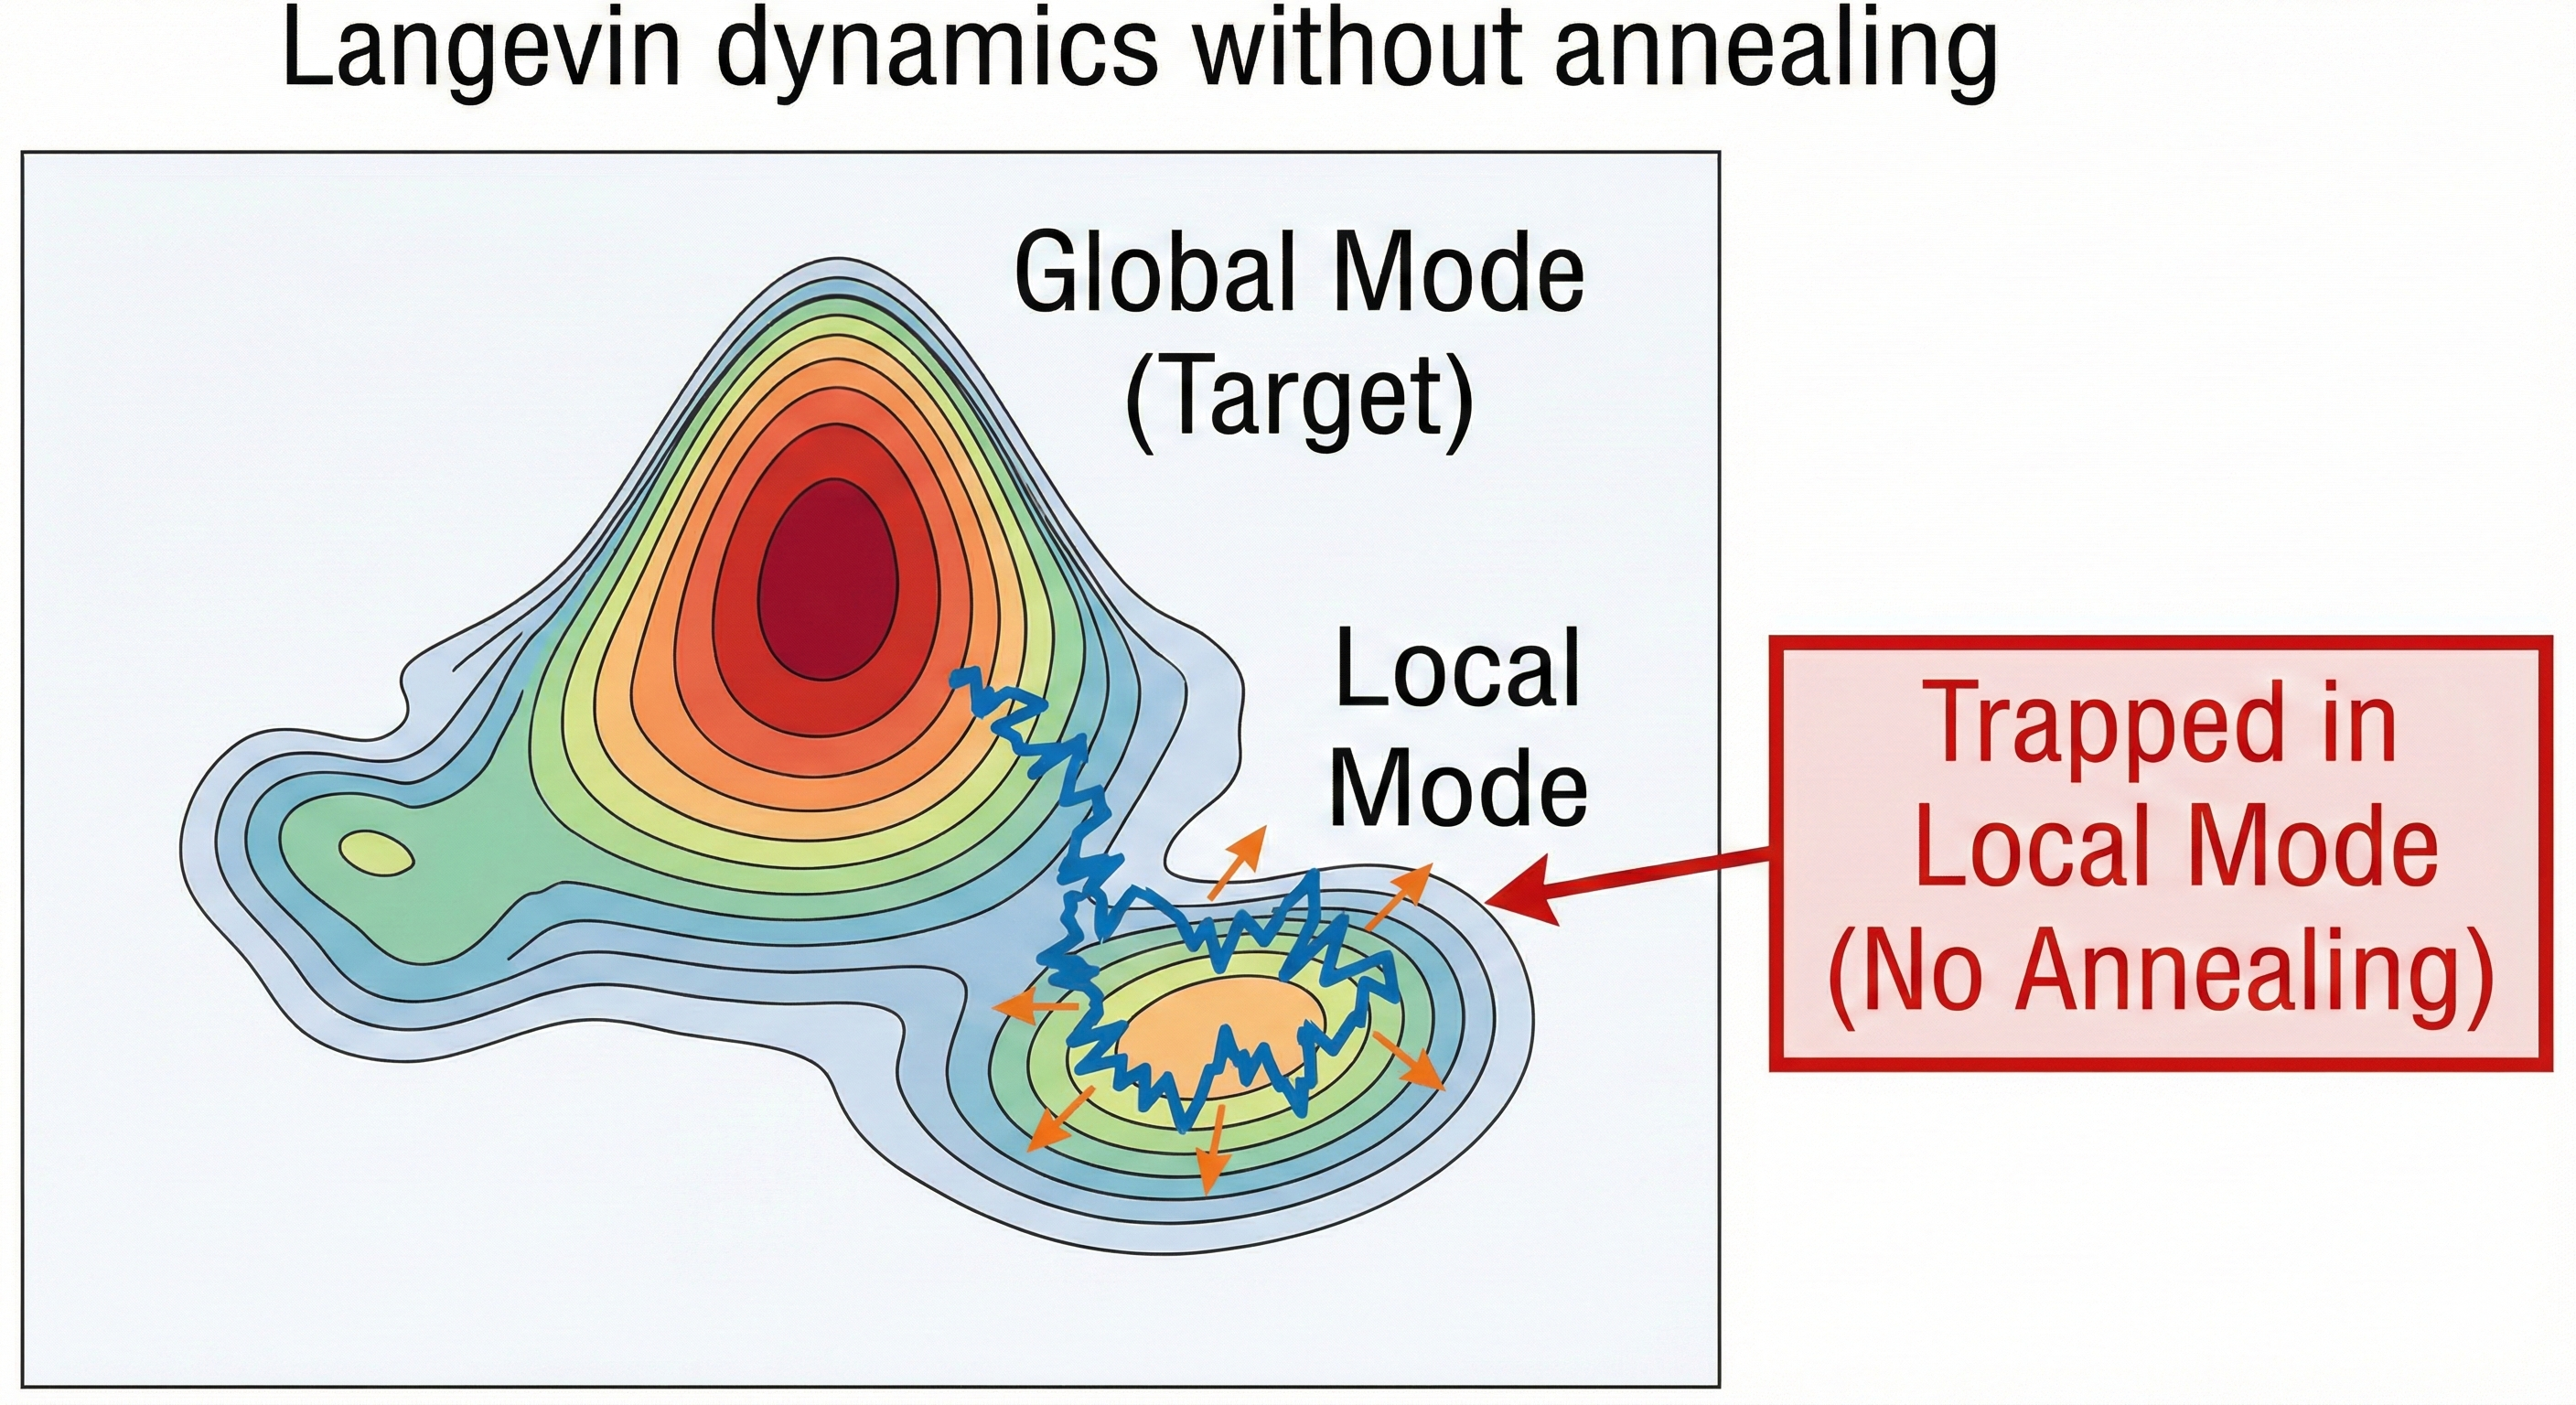
\includegraphics[width=0.9\textwidth]{../Common_Images/pnp/langevin-annealing.png}
    \caption{Without annealing, Langevin dynamics can become trapped in local modes, limiting posterior exploration and sample diversity. Image generated with Nano Banana Pro}
    \label{fig:langevin_annealing_traps}
\end{figure}

This specific connection is remarkable. It shows that by injecting controlled noise into PnP/RED algorithms, and using denoisers evaluated across multiple noise levels $\sigma$ to guide the random walk, we transition from classical deterministic solvers to stochastic samplers. This exact derivation forms the mathematical backbone of modern \textbf{Score-Based Generative Models} and \textbf{Diffusion Models}.

\subsection{Annealed Langevin Dynamics and Diffusion Posterior Sampling}
\label{sec:annealed_langevin}

While Equation \eqref{eq:langevin_pnp} elegantly links PnP, RED, and Langevin sampling, running this algorithm at a \emph{fixed} noise level $\sigma$ presents a massive practical challenge. The true posterior distribution of natural images is highly multi-modal -- it consists of many sharp peaks separated by vast regions of near-zero probability. 

\begin{figure}[htbp]
    \centering
    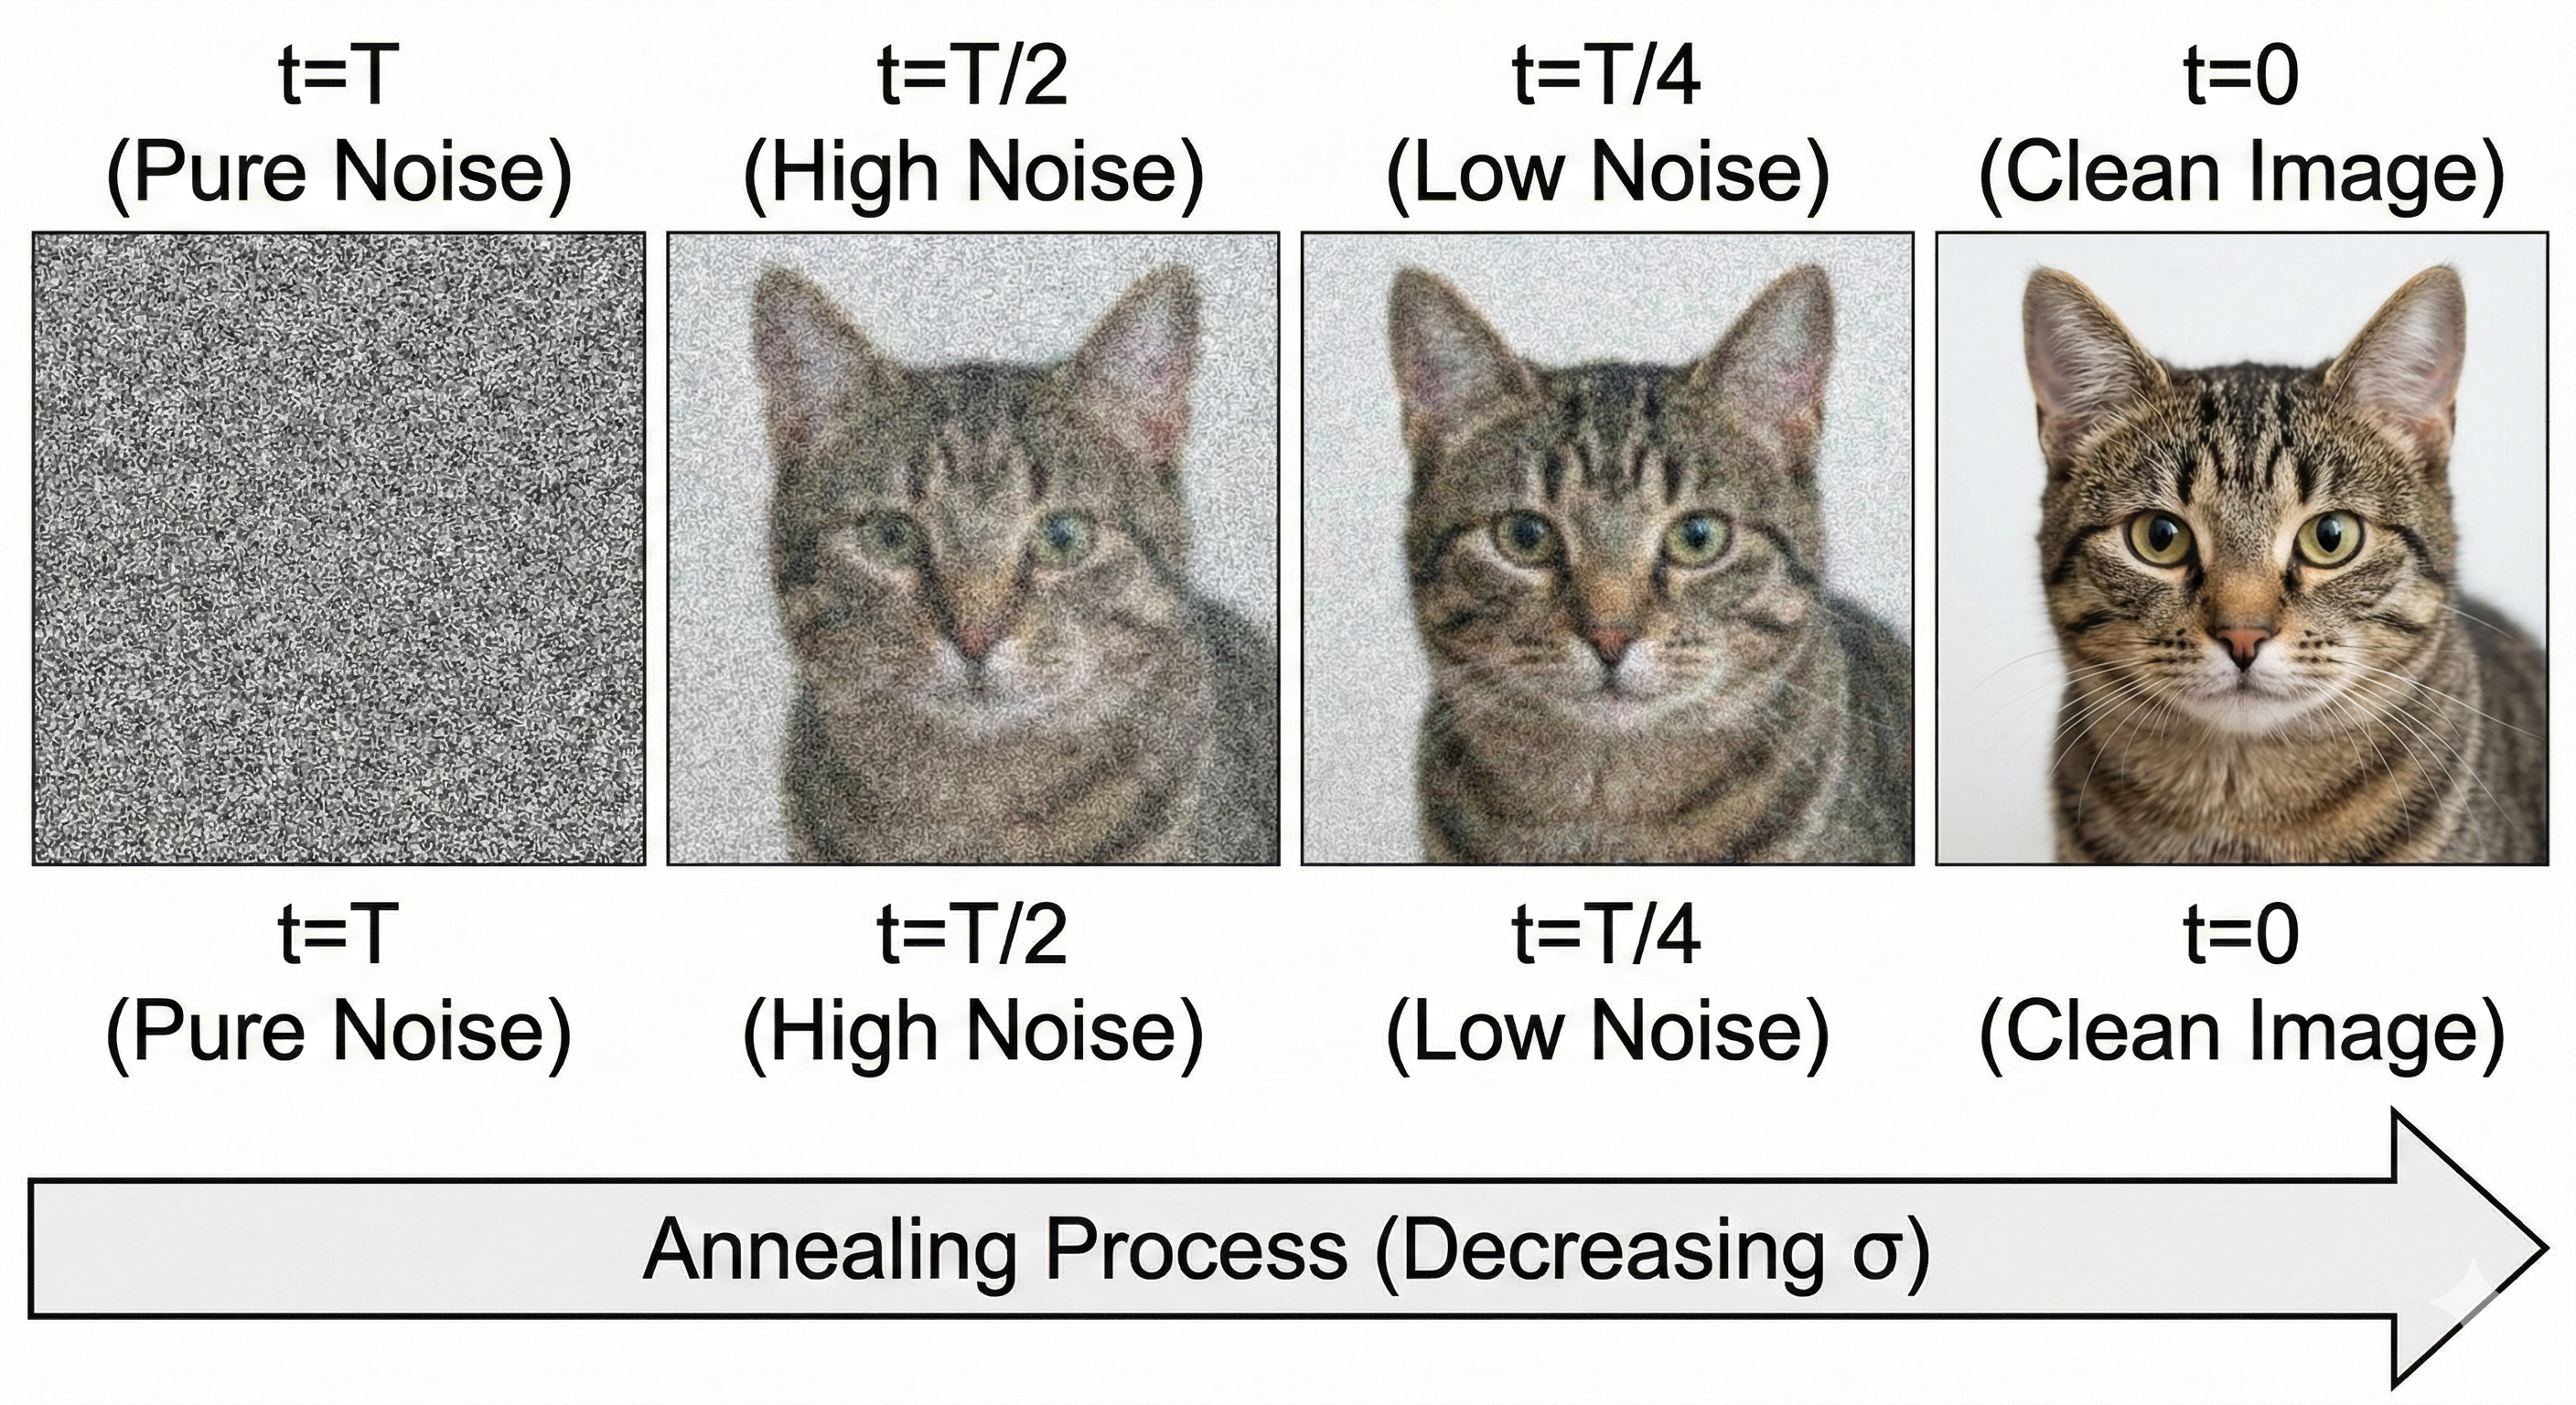
\includegraphics[width=0.9\textwidth]{../Common_Images/pnp/noise-schedule.png}
    \caption{Annealed noise schedule used in diffusion models: sampling starts from high-noise Gaussian states and progressively refines toward clean image structure as the noise level decreases. Image generated with Nano Banana Pro.}
    \label{fig:noise_schedule_diffusion}
\end{figure}

If we run standard Langevin dynamics with a small $\sigma$, the random noise $\sqrt{\tau} z_k$ is not strong enough to kick the image out of a local peak. The algorithm gets trapped, failing to explore the full diversity of the posterior. Conversely, if we use a very large $\sigma$, the image wanders freely but never settles into a sharp, high-quality solution.

Modern score-based generative models and diffusion models solve this fundamental issue by introducing a \emph{noise schedule}. Instead of a fixed $\sigma$, we define a decreasing sequence of noise levels $\sigma_T > \sigma_{T-1} > \dots > \sigma_1 > \sigma_0 \approx 0$. 

We then train a single, time-dependent neural network denoiser, $D_{\sigma_t}(u)$, capable of estimating the score at any noise level. The sampling process begins at $t=T$ with pure Gau\ss ian noise. At each step $t$, we run the Langevin update \eqref{eq:langevin_pnp}, but we dynamically update the noise level and step size $\tau_t$, i.e.,
\begin{align}
    u_{t-1} = u_t - \frac{\tau_t}{2} \nabla_u F(K u_t, f^\delta) + \frac{\tau_t}{2\sigma_t^2} \Big( D_{\sigma_t}(u_t) - u_t \Big) + \sqrt{\tau_t} z_t \, .
    \label{eq:dps_update}
\end{align}
This process is known as \textbf{Annealed Langevin Dynamics}. At high noise levels (large $\sigma_t$), the probability landscape is heavily smoothed, allowing the iterates to freely move toward the general region of valid solutions. As $t$ decreases, the landscape sharpens, and the algorithm fine-tunes the details.

When applied to inverse problems, this specific interleaved update -- taking a gradient step for data consistency $-\nabla_u F(K u_t, f^\delta)$ combined with an annealed score step -- is widely known as \textbf{Diffusion Posterior Sampling (DPS)} \cite{chung2023diffusion}. By looking at \eqref{eq:dps_update}, we can finally appreciate the complete evolution of this field:
\begin{itemize}
    \item \textbf{PnP / RED:} Set $\sigma_t$ to a constant (or a simple heuristic decay), drop the random noise $z_t$, and aim for a single consensus equilibrium.
    \item \textbf{DPS / Diffusion:} Rigorously anneal $\sigma_t$ down to zero, keep the stochastic noise $z_t$, and generate a full distribution of highly detailed, diverse posterior samples.
\end{itemize}
Ultimately, replacing proximal operators with denoisers was not only an algorithmic trick, but lead to the discovery of a mathematical interface connecting variational optimisation, fixed-point theory, and stochastic generative modelling.

\section{Summary}

In this chapter, we have transitioned from explicit regularisation functionals to implicit ones, discovering the deep mathematical connections between classical inverse problems, fixed-point theory, and modern generative AI:
\begin{itemize}
    \item \textbf{Plug-and-Play (PnP)} allows us to effortlessly replace the proximal operator in algorithms like HQS and ADMM with state-of-the-art neural network denoisers. By extending this to strictly constrained formulations (\textbf{PnP-Bregman}), we can leverage iterative regularisation to naturally restore fine details without relying on heuristic noise-decay schedules.
    \item \textbf{Theoretical Convergence} of these methods requires a paradigm shift. Because standard denoisers lack symmetric Jacobians, classical optimisation proofs break down. We must either strictly constrain network architectures to act as valid proximal operators (the optimisation perspective) or rely on Lipschitz continuity and the Krasnosel'skii-Mann theorem to guarantee convergence to a consensus equilibrium (the fixed-point perspective).
    \item \textbf{Regularisation by Denoising (RED)} attempts to construct an explicit variational functional from the denoiser. While theoretically flawed as an optimisation problem due to the asymmetric Jacobians of deep networks, it mathematically converges as a highly robust root-finding algorithm (FP-RED).
    \item \textbf{Tweedie's Formula and Score Matching} provide the probabilistic theory. By proving that optimal MMSE denoisers compute the score function (the gradient of the log-probability), we reveal that PnP and RED are implicitly performing gradient ascent on the data distribution. 
    \item \textbf{Langevin Dynamics and DPS}: By injecting stochastic noise into our algorithms and utilising an annealed noise schedule, we transition from deterministic solvers that seek a single MAP estimate to \textbf{Diffusion Posterior Sampling (DPS)}. This unlocks the ability to sample the full posterior distribution, bridging classical iterative methods with the stochastic sampling techniques of modern Diffusion Models.
\end{itemize}